\chapter{Codebase: List Panel}

The list panel is the central element in the 'explorer' tab.  It
houses either:

\begin{enumerate}
  \item The results of the search done from the search box.
  \item The contents of the container selected in the object tree
\end{enumerate}

\section{Description}

The listpanel is a fixed-width list of items with each item having a
set of action buttons which can be configured while setting up the
widget.  It has its own scrollable field of view.

As explained earlier, the listpanel contains either search results or
contents of the container element selected in the object tree.  For
each such element, there is a helpful icon which uniquely identifies
the data-type (block, segment etc.) of the item in question.  Also,
there is an 'Add' button.  Clicking this add button adds the data-item
to the 'basket' instance for the current session.  The basket will be
discussed later.

\subsection{Filtering}

In some instances, there are simply too many results in the
list-panel.  In times like this, it is helpful to filter the results
by data-type.  The 'change' button on the top-right does just that.
It allows you to select the data-types you want to see and thus narrow
your search.

\subsection{Interface transformations}

When hovering over a data-item, it is highlighted so as to allow one
to visually assess the correct button to be clicked as well as the
icon.

\begin{figure}[h!t]
  \centering
  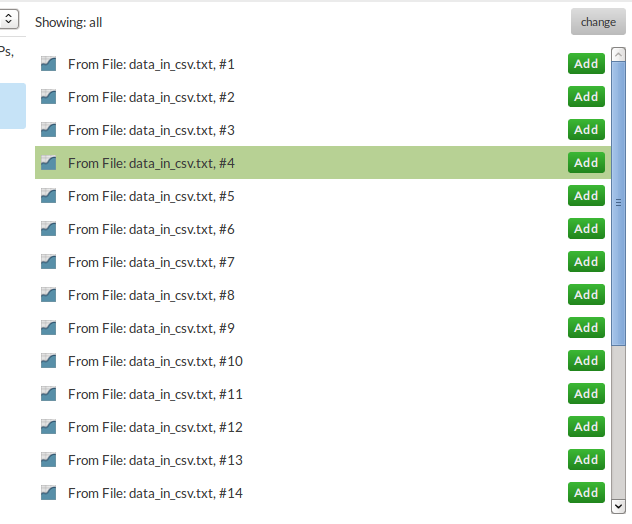
\includegraphics[width=\textwidth]{src/images/wdat-list-panel.png}
  \caption{ListPanel}
\end{figure}

\section{Methods}

There are a few methods exposed by the wdat.listpanel module.

\begin{enumerate}
  \item{wdat.listpanel.filter()} \hfill \\
  Filter items based on a list of valid data-types specified as an
  argument.  Also results in immediate rendering of the filtered
  items.

  \item{wdat.listpanel.data()} \hfill \\
  Allows clients to get/change the data within the listpanel module.
  Used, for example, by the search bar to update the list.

  \item{wdat.listpanel.render()} \hfill \\
  Clears the GUI for the list panel and rewrites the interface again.
\end{enumerate}
